\chapter{Technical Characteristics} \label{ch:technical-characteristics}

Both dashboard generations operate from the vehicle's 9--16~V electrical system.
Replica Next draws approximately 13~mA from the battery while powered down, whereas the classic Replica consumes no standby current when fully switched off.

\section{Measurement Capabilities}

\begin{itemize}
    \item \textbf{Vehicle speed:} measured through the mechanical or electronic speed sensor.
          The absolute error is 10~km/h, the relative error 3~km/h, and the indication saturates at 999~km/h (or mph for imperial units).
    \item \textbf{Engine speed:} derived from the ignition signal via an RC-limited optocoupler stage (430~nF/1.2~k\ohm{} with diode clamping).
          The absolute and relative errors are within 200~rpm.
    \item \textbf{Fuel level:} read from the resistive tank sender with an uncertainty of approximately 10~litres.
    \item \textbf{Coolant temperature:} displayed qualitatively using the OEM thermistor connected through the vehicle harness.
    \item \textbf{Time:} maintained to within one minute.
          Replica employs a DS3231 real-time-clock module with a CR2032 backup cell; Replica Next keeps time through firmware.
    \item \textbf{Indicator lamps:} direction indicators, high beam, oil pressure warnings, generator status, handbrake, rear window heating or diesel glow-plug, and front/rear fog lights.
\end{itemize}

\chapter{Operating Conditions and Safety Precautions} \label{ch:operating-conditions}

\section{Environmental Limits}

\begin{itemize}
    \item Ambient operating range: \(-40\,^{\circ}\mathrm{C}\) to \(+70\,^{\circ}\mathrm{C}\) with up to 95\% relative humidity.
    \item Year-round use inside the passenger compartment is supported, including long-term parking.
    \item Store the dashboard inside the vehicle cabin or in a dry indoor space between \(+15\,^{\circ}\mathrm{C}\) and \(+40\,^{\circ}\mathrm{C}\), protected from direct sunlight.
\end{itemize}

\section{Responsibilities and Limitations}

\begin{itemize}
    \item Digifiz dashboards are enthusiast devices intended for project cars; they are not certified measuring instruments.
    \item Installations are performed at the owner's risk.
          When readings appear questionable, verify them with factory gauges or independent instruments.
    \item Do not feed Digifiz measurements into automated vehicle control systems.
    \item The authors guarantee the documented functionality during a one-year warranty period for installations performed jointly and for two weeks on self-installations; malfunctions within these windows will be repaired.
\end{itemize}

\chapter{Preparation for Work and Work Order} \label{ch:preparation}

\section{Preparing the Vehicle}

Follow the sequence below when replacing the factory cluster:
\begin{enumerate}
    \item Remove the plastic trim covering the pedals and dashboard to expose the instrument cluster.
    \item Disconnect the vehicle battery.
    \item Unplug the factory harness from the instrument panel.
    \item Disconnect the mechanical speedometer cable (if fitted).
    \item Unscrew the cluster from its brackets and carefully remove it from the vehicle.
    \item Route the temperature and speed sensor harnesses supplied with the Digifiz kit.
    \item Install the new dashboard into the bracket grooves and secure it with screws.
    \item For Replica Next, connect the Volkswagen MFA sensors or compatible replacements and route the cables to the CE~1/CE~2 connectors.
    \item On single-connector variants (\texttt{GACS}/\texttt{GARS}/\texttt{DARS}/\texttt{DACS}), manually connect the labelled MFA\_MODE, MFA\_RESET, MFA\_BLOCK, and handbrake wires if the vehicle harness lacks these contacts.
    \item Plug in the harness(es) and connect the electronic speed sensor or speedometer cable as required.
    \item Reinstall the dashboard trim and pedal cover in the reverse order.
\end{enumerate}

\section{Working with the Instrument Panel}

The dashboard powers up automatically with ignition.
During the self-test the speed scale illuminates fully before stabilising at the current RPM value; the sidelights control the backlight.
Once the vehicle begins moving, the MFA controller updates the measurements described in \Cref{ch:technical-characteristics}.

\section{MFA Functions}

Six MFA pages are available:
\begin{enumerate}
    \item Daily operating time.
    \item Trip distance.
    \item Fuel consumption (not implemented on the first Replica revision).
    \item Average speed (displayed as the value multiplied by ten).
    \item Engine oil temperature (external harness required).
    \item Ambient temperature (external harness required).
\end{enumerate}

On classic Replica dashboards a capacitive touch point behind the VW badge cycles the pages.
Replica Next relies on an external steering column switch.
Touch durations behave as follows:
\begin{itemize}
    \item Short press (\(<1\)~s): cycle to the next MFA function.
    \item Medium press (1--3~s, when no steering column switch is present): switch between MFA memory blocks.
    \item Long press (3--7~s): reset the active MFA function (affecting consumption, trip distance, elapsed time, and average speed).
\end{itemize}

\section{Backlight Control and Indicator Layout}

Classic dashboards provide a manual brightness trim above the parking-light switch, whereas Replica Next relies on automatic brightness using an onboard photodiode.
Automatic control can be overridden through configuration commands described in \Cref{ch:replica-next-setup}.

The layout of the horizontal indicator block and the on-screen labelling are shown in \Cref{fig:indicator-layout,fig:indicator-legend}.

\begin{figure}[htbp]
    \centering
    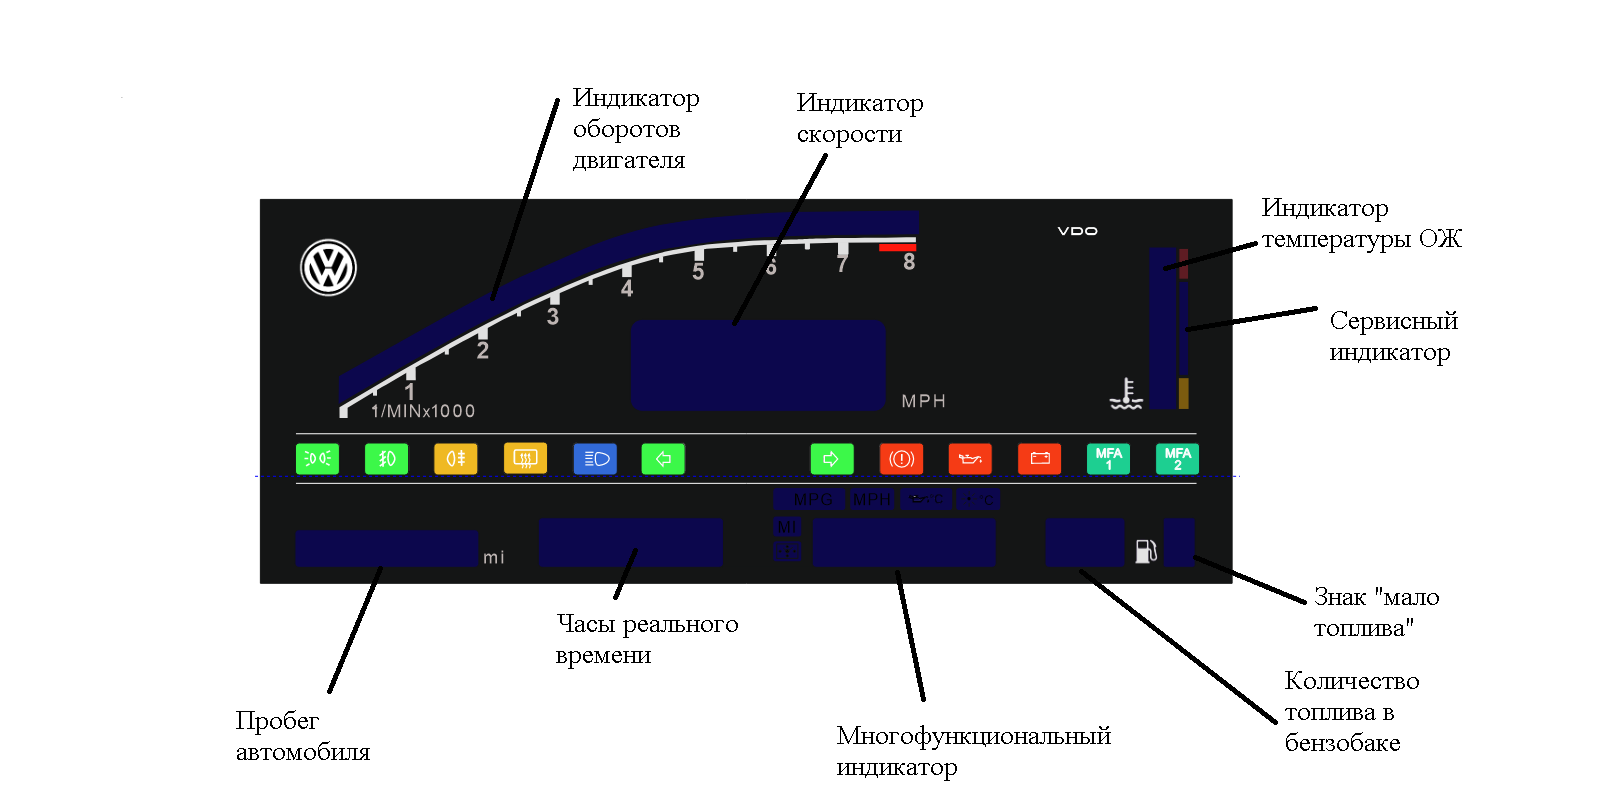
\includegraphics[width=0.85\textwidth]{digifiz_manual/image017.png}
    \caption{Indicator layout displayed during the power-on self-test.}
    \label{fig:indicator-layout}
\end{figure}

\begin{figure}[htbp]
    \centering
    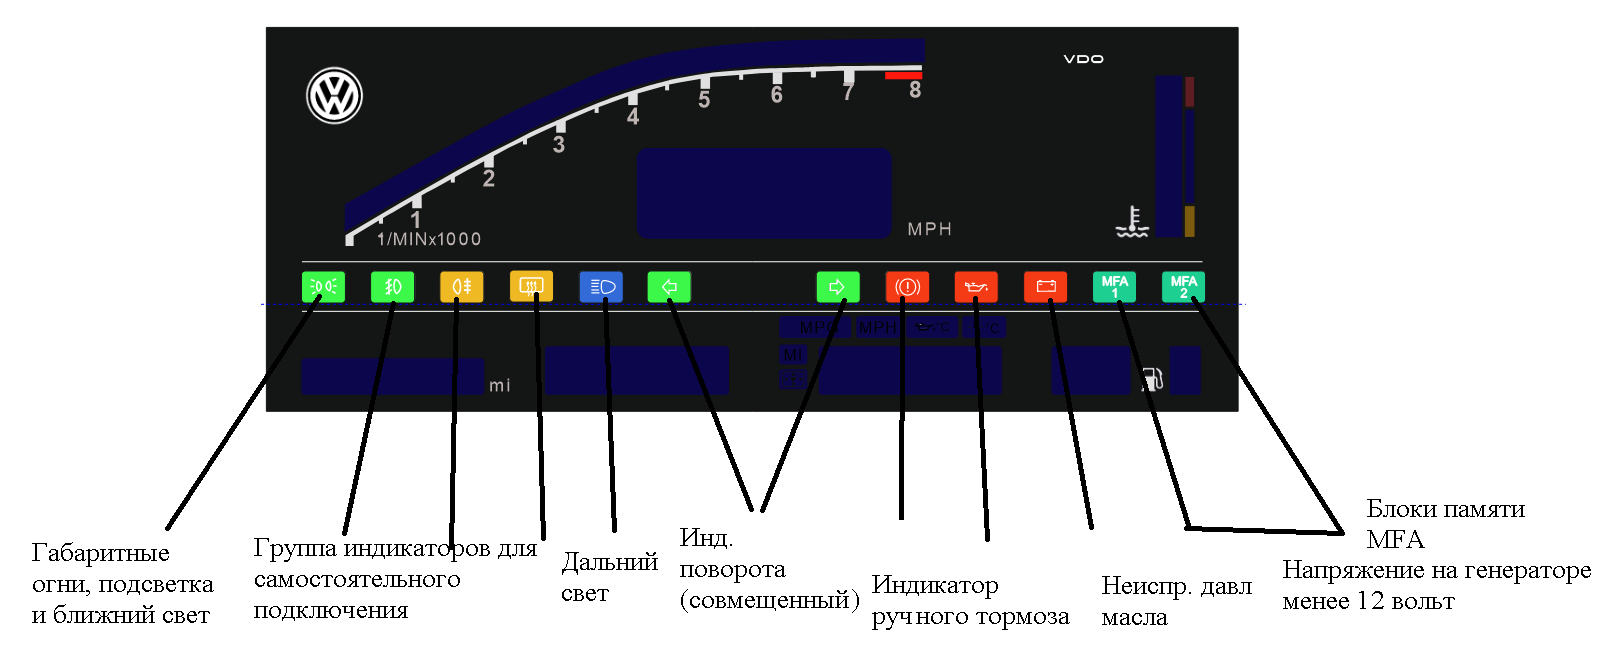
\includegraphics[width=0.8\textwidth]{digifiz_manual/image018.png}
    \caption{Legend for the horizontal indicator group.}
    \label{fig:indicator-legend}
\end{figure}

\section{Configuration Interfaces}

Both generations provide maintenance interfaces:
\begin{itemize}
    \item Classic Digifiz Replica units include a Bluetooth 2.0 (or BLE-compatible) module.
          Install the \emph{Serial Bluetooth Terminal} application from Google Play, pair with the dashboard, and issue commands directly from the terminal view.
          Apple iOS devices cannot connect to the module.
    \item Replica Next exposes an embedded Wi-Fi access point that serves the configuration portal detailed in \Cref{ch:replica-next-setup}.
          Disable mobile data while connecting to ensure the captive portal loads correctly.
\end{itemize}

Both generations also accept configuration commands over the USBasp programming interface when the dashboard is connected to a computer, which powers the unit for bench testing.
